\documentclass{article}
%\usepackage{tgadventor}
%\renewcommand*\familydefault{\sfdefault} %% Only if the base font of the document is to be sans serif
%\usepackage[T1]{fontenc}

\usepackage[default]{comfortaa}
\usepackage[T1]{fontenc}
\usepackage{graphicx}
\usepackage{xcolor}
\usepackage[some]{background}
\usepackage{geometry}
\usepackage{hyperref}
\usepackage{caption}
\usepackage{subcaption}
\urlstyle{same}

\definecolor{titlepagecolor}{cmyk}{1,.60,0,.40}

\backgroundsetup{
scale=1,
angle=0,
opacity=0.1,
contents={\begin{tikzpicture}[remember picture,overlay]
 \path [fill=titlepagecolor, opacity=1] (-0.3\linewidth,-2) rectangle (0.3\linewidth,3);
 \path [fill=titlepagecolor, opacity=0.8] (-0.45\linewidth,-4.75) rectangle (0.45\linewidth,5.75);
 \path [fill=titlepagecolor, opacity=0.6] (-0.6\linewidth,-7.5) rectangle (0.6\linewidth,8.5);
 \path [fill=titlepagecolor, opacity=0.4] (-0.75\linewidth,-10.75) rectangle (0.75\linewidth,11.25);  
 \path [fill=titlepagecolor, opacity=0.2] (-0.9\linewidth,-14) rectangle (0.9\linewidth,14);
\end{tikzpicture}}
}


\begin{document}
    %\begin{titlepage}
    %    \title{Where should a board game caf\'{e} be located in Turku?}
    %    \author{Tom Bullock}
    %    \date{}
    %    \maketitle
    %    \thispagestyle{empty}
    %\end{titlepage}

    \begin{titlepage}
        \begin{center}
            \vspace*{0.45\textheight}
            \begin{minipage}{0.6\linewidth}
                \BgThispage
                \centering
                {\huge \textcolor{white}{Where should a board game caf\'{e} be located in Turku?}}
            \end{minipage}
        \end{center}

    \null\vfill
    \vspace*{1cm}
    \noindent
    \hfill
    \begin{minipage}{0.35\linewidth}
        \begin{flushright}
            {\large \textcolor{white}{Tom Bullock}}
        \end{flushright}
    \end{minipage}
    %
    \begin{minipage}{0.02\linewidth}
        \textcolor{white}{\rule{1pt}{25pt}}
    \end{minipage}
    \end{titlepage}

    \abstract{
        This report aims to answer the question ``which districts in the city of Turku would be best suited for a board game caf\'e?'' 
        As a city with a high number of board game players, and the nearest board game caf\'es being over two hours travel away, there is a noticeable gap in the market, and finding the right spot would prove incredibly lucrative.
        This question was answered by studying venue features within the vicinity of board game caf\'es around Europe, as well as the centres of major cities that do not possess them, and using these to train several classification models.
        After determining the best model, it was then used to determine the feasibility of each district of Turku, with these feasibilities visualised by a choropleth map. 
    }

    \newpage

    \tableofcontents

    \newpage

    \section{Introduction}

    \subsection{Background}

    The city of Turku in the southwest of Finland has a large fan base for board games: with a population of 191,331, it possesses three brick and mortar board game shops, along with a dedicated board game section in most toy and book shops, and even a board game loan scheme at the public library. 
    To put this in perspective, this is the same number of shops as the capital city Helsinki, whose population of 648,042 far exceeds that of Turku's. 
    And yet, despite this, Turku does not possess a board game caf\'e, a place where people can socialise, eat, drink and play games or run tabletop campaigns together. 
    Given that Turku is also in possession of over a dozen escape rooms (an activity with a significant overlap in terms of customers), there is clearly no lack of demand for opportunities to play games together.\\

    The closest cities to Turku that possess board game caf\'es are Helsinki and Tampere, both of which are located over two hours away, and so do not fill this niche; as a result, anyone who opens a board game caf\'e would certainly find it a lucrative venture.
    
   % Such a café would likely prove very lucrative within Turku as the closest board game cafés are located in Helsinki and Tampere, both being two hours distance away, and so the main question for a prospective café owner to ask is which neighbourhood of Turku would be most likely to succeed? This project intends to answer that by analysing the locations of board game cafés around Europe, as well as centres of major cities that don't have any board game cafés, and determining via a logistic regression model which neighbourhoods in Turku would be best suited for housing such a café. This research will be performed with the use of the FourSquare API in order to perform venue queries based on geographical data.

    \subsection{Problem}

    The goal of this project is to determine within which districts of Turku a board game caf\'e would be most suitable.
    This will be done by considering venue data, obtained via the Foursquare Places API, in the vicinity of board game caf\'es within Europe, as well as for the centres of the largest cities in Europe that do not have a board game caf\'e.
    As a leisure venue, it seems reasonable to believe that a board game caf\'e's location would largely depend on the amenities within its vicinity; it is more likely to be found in a younger, more affluent area, and this would manifest in the sorts of venues there.

    
    \subsection{Interest}

    Given that there is a gap in the market within Turku for a board game caf\'e, being able to determine which districts are likely to be suitable allows a prospective caf\'e owner to make a more informed decision on where would be worth investigation. 
    In the case of there being a huge difference in the cost of renting space between districts, this information will allow this prospective owner to optimise their decision in terms of the likelihood of suitability and cost, making them more likely to survive.

    \section{Data Acquisition}

    \subsection{Data sources}

    The training data used for this project consists of venue data retrieved from the Places API provided by Foursquare%
    \footnote{
        \url{https://foursquare.com/products/places/}
    }%
    ; this API requires longitudinal and latitudinal data for locations that are of interest, and we considered any venue within a 400m radius of these points. 
    In particular, we will restricted ourselves to locations within Europe.
    The reason for this is that cities in different parts of the world follow very different patterns in terms of congregations of shops and services (an example of this is the difference between Europe and North America in terms of suburban shopping), and Finland is very much a Nordic country, with the structure of its cities being most similar to the Scandinavian nations, Estonia and Iceland.
    However, restricting ourselves to just these countries would leave us with a severely limited data size, making it difficult to build an extendable model. 
    To that end, the decision to work with European locations allows for a larger data set without veering too far from the city planning styles of the Nordic nations.\\
    
    The locations of board game caf\'es were given in an extensive list, by Andy Matthews at Meeple Mountain, of board game caf\'es around the world \cite{Meeple}.
    The caf\'es were placed into a Google Map \cite{MeepleMap}, from which a kml file containing every caf\'e and its address could be extracted.\\

    For the major cities we made use of the list of the five hundred largest cities in Europe as provided by the City Mayors website \cite{CityMayors}, as well as the largest cities (over 149,000 people to match the smallest values within the City Mayors list) within Turkey \cite{WikiTurkey} because this country is a sovereign state within Europe but was omitted from the City Mayors list.\\

    With the locations of board game caf\'es, as well as additional major cities, in Europe we made use of OpenStreetMap's Nominatim search engine%
    \footnote{
        \url{https://nominatim.openstreetmap.org/ui/search.html}
    }%
    , by way of the geopy python pacakge, to obtain the longitudinal and latitudinal data of each street address.\\

    The data for the districts of Turku was collected in a similar fashion, starting with the list of districts found upon Wikipedia \cite{WikiTurku}, from which we obtained geographical data via geopy queries, and finally venue data by querying the Foursquare Places API. 
    In addition, for later visualisation, the OpenStreetMap ID number for each district was retrieved, as this could be used with the OpenStreetMap polygons website%
    \footnote{
        \url{http://polygons.openstreetmap.fr/index.py}
    }%
    to generate the district outlines in json format.

    \subsection{Data cleaning}

    Given that data was collected from multiple sources, it comes as no surprise that a fair amount of data cleaning was needed.\\
    
    In order to restrict ourselves to European caf\'es, and because the data within Matthews' list does not include continents, we made use of the Wikipedia list of European countries \cite{WikiEU} to automatically filter the caf\'es: if a caf\'e's country belongs to the list of sovereign states in Europe then it is included within our training data.
    In some cases this required relabelling some countries, as Wikipedia considers the United Kingdom as a single entity, whereas Matthews' list separates it into its constituent countries.
    In addition, Matthews' list does not contain any board game caf\'es within Russia, but after subsequent venue searches the caf\'e Chil Angart in Karsnodar was found, and so this was added to the list of caf\'es, whilst Krasnodar was removed from the list of cities.
    Upon querying the board game caf\'e list with geopy it was found that 52 of the venues did not provide longitudinal and latitudinal data, and this was down to a number of issues ranging from OpenStreetMap and Google Map not agreeing on addresses/street maps, OpenStreetMap not being granular enough or not providing locations with the Latin alphabet, or the provided location was simply incorrect or did not exist.
    It was also found that there existed duplicates of some venues with the differences being difficult to automate the correction of.
    Whilst duplicates and incorrectly-given values were deleted, the rest were corrected by hand, as the list of cafe\'es contained around 300 elements and so these errors amount to a large percentage of overall data points. \\

    For the city data there contained some small issues: firstly, the city of Rome was given in Italian (Roma) and so when we wanted to compare it to the list of caf\'es it was not immediately removed despite Rome containing a board game caf\'e. 
    Secondly, a number of British counties were included within the list, with some containing no single large hub of people, and so counties were removed from the list; this amounted to removing ten items out of a list of over 500 and so no significant loss, especially as the United Kingdom was already well represented.
    In addition to this, Turku was removed from this list, as it made no sense to train the model with the city we wish to investigate.
    Thirdly, there were some locations that did not give results when querying geopy, or provided incorrect locations (an example of this is Van, Turkey, which Nominatim treated as short-hand for Vietnam); these locations were corrected by hand to prevent a further reduction in data.
    Finally, a number of the cities included in Russia technically belong to the continent of Asia (those in central or eastern Russia), and so any cities to the east of the Ural mountains were omitted.\\

    After collecting venue data for both of these sets of locations, any instances of board game caf\'es appearing within their own or neighbouring sets of venues were removed as best as possible; this was done by removing instances of caf\'e names within venues, with some words replaced e.g. `caf\'e' and `cafe', and in other instances places removing venues with the Foursquare category ID corresponding to `gaming caf\'e' (4bf58dd8d48988d18d941735)%
    \footnote{
        A full list of category IDs can be found at \url{https://developer.foursquare.com/docs/build-with-foursquare/categories/}.
    }%
    .
    In the case of the city list, any venues that matched that ID were checked and either replaced with a correct ID and category name (in the case of arcades and betting shops, etc.) or were removed if they were found not to exist.\\

    For the Turku data, whilst the geopy queries always retrieved values, they did not always provide the correct ones for our purposes. 
    This was due to geopy providing a single result whenever a query was made, but there being more than one when compared against the Nominatim search; an example of this is District VII in Turku, where performing the (necessarily truncated) search `VII Turku' in Nominatim provides the administrative region as well as a terminal in Turku's main train station. 
    Since these regions were needed the offending regions needed to be corrected by hand, as well as the removal of the airport because it did not provide any regional data.


    \subsection{Feature selection}

    Once the data had been cleaned, there were 62,674 samples in the training data and 5,916 in the Turku data.
    The training data was combined and its venue category name data was one-hot encoded; these encodings were then grouped together in terms of caf\'e and city for those near a board game caf\'e (the inclusion of the city to prevent grouping venues near caf\'es with the same name but different location) and in terms of city for those that are not.
    After grouping the mean was taken for each encoding, so that each caf\'e and city was left with a vector of values between zero and one, where each value provides the percentage (as a decimal) that particular venue category takes up of the venues in that area.
    These vectors were then together combined into a numpy array (of arrays) that was scaled using a standard scaler so that the models would not be using comparatively small values.
    A standard scaler was used in particular to ensure that negative numbers would not arise, which in preliminary tests caused problems.\\

    The Turku data was put through an identical process of encoding, grouping and scaling, with the encoder and scaler being the ones fit with the training data to ensure that the values within the Turku data were not only of similar scale to those in the training data, but so that the encoded data corresponded to the same venue categories and hence did not lead to misleading results.


    \section{Exploratory Data Analysis}

    \subsection{Geographical analysis of board game caf\'es}

    \begin{figure}[t]
        \centering
        \begin{subfigure}{0.49\textwidth}
            \centering
            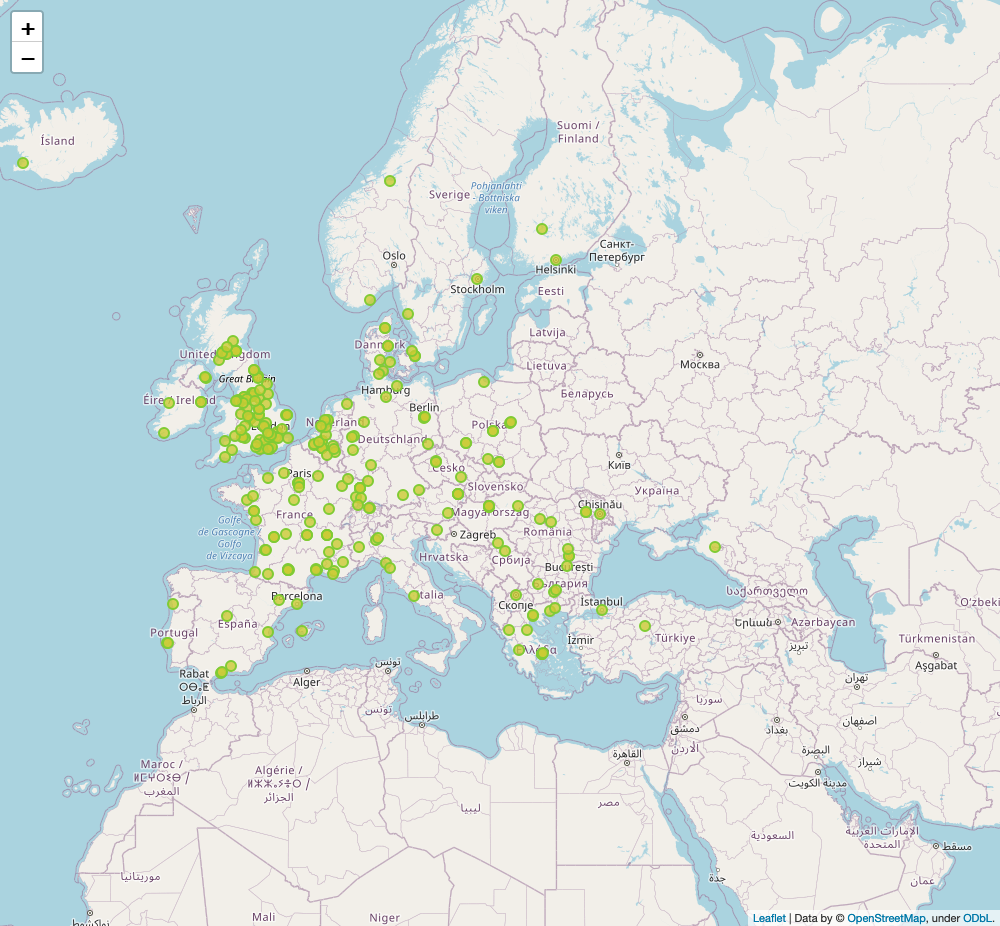
\includegraphics[width=\textwidth]{Map_eu_cafe.png}
            \caption{\label{fig:MapEUCafe}A map of each board game caf\'e within Europe.}
        \end{subfigure}
        \hfill
        \begin{subfigure}{0.49\textwidth}
            \centering
            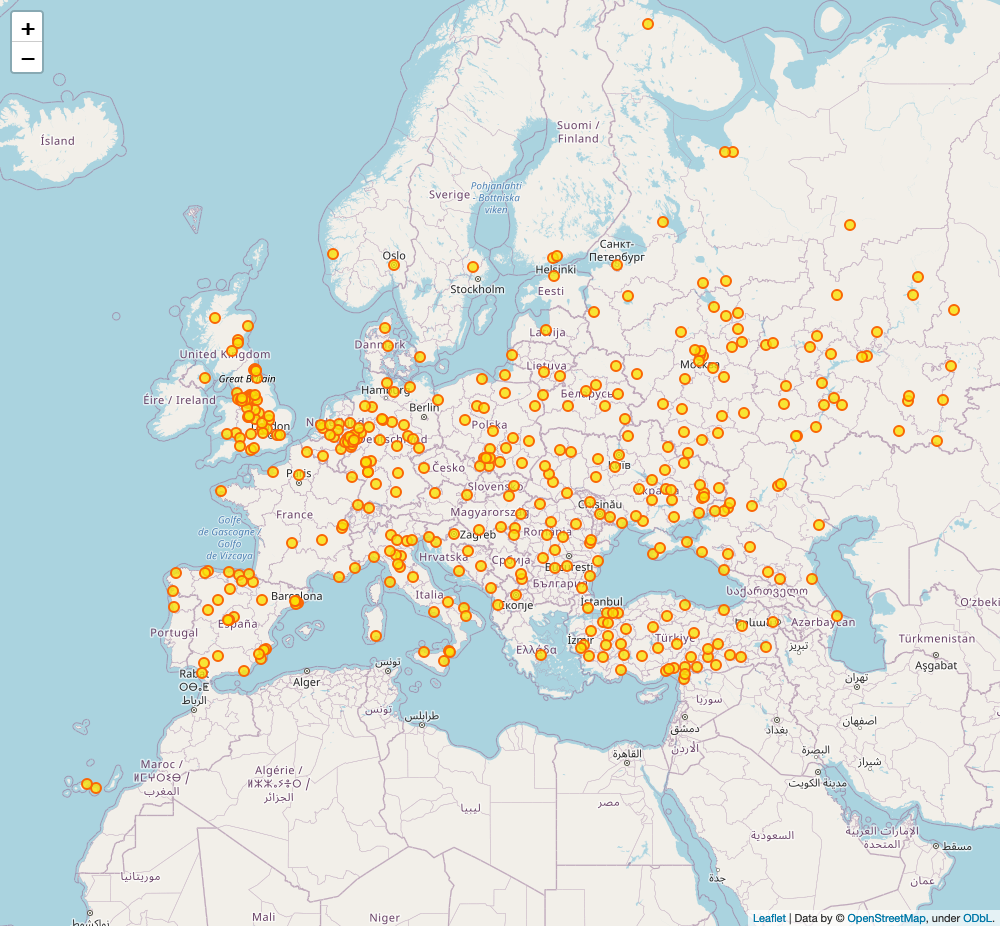
\includegraphics[width=\textwidth]{Map_eu_cwc.png}
            \caption{\label{fig:MapEUCity}A map of each major city within Europe without a board game caf\'e.}
        \end{subfigure}
        \caption{\label{fig:MapEUComp}Comparative maps of board game caf\'e locations and major cities without.}
    \end{figure}

    The caf\'es and cities were plotted (see Figure \ref{fig:MapEUComp}), and some points quickly become apparent.
    Firstly, there are only a small number of both board game caf\'es and larger cities within the Nordic nations, so we were justified in considering Europe as a whole, with the alternative being to consider smaller cities within the Nordic nations and have very skewed data towards places without board game caf\'es.
    Secondly, the number of board game caf\'es within eastern Europe is very small, in particular within Russia and the Baltic region, whereas in countries like France, Denmark, the Netherlands and the United Kingdom there are are similar numbers of caf\'es to cities without them (and in the case of France and the Netherlands there are far more caf\'es).
    Further to this, there are comparatively few caf\'es in Spain and Italy.
    This suggests that there is a higher demand for board game caf\'es in colder, more (culturally) western European countries, which Finland qualifies as.

    \subsection{Comparison of venues}

    \begin{figure}[t]
        \centering
        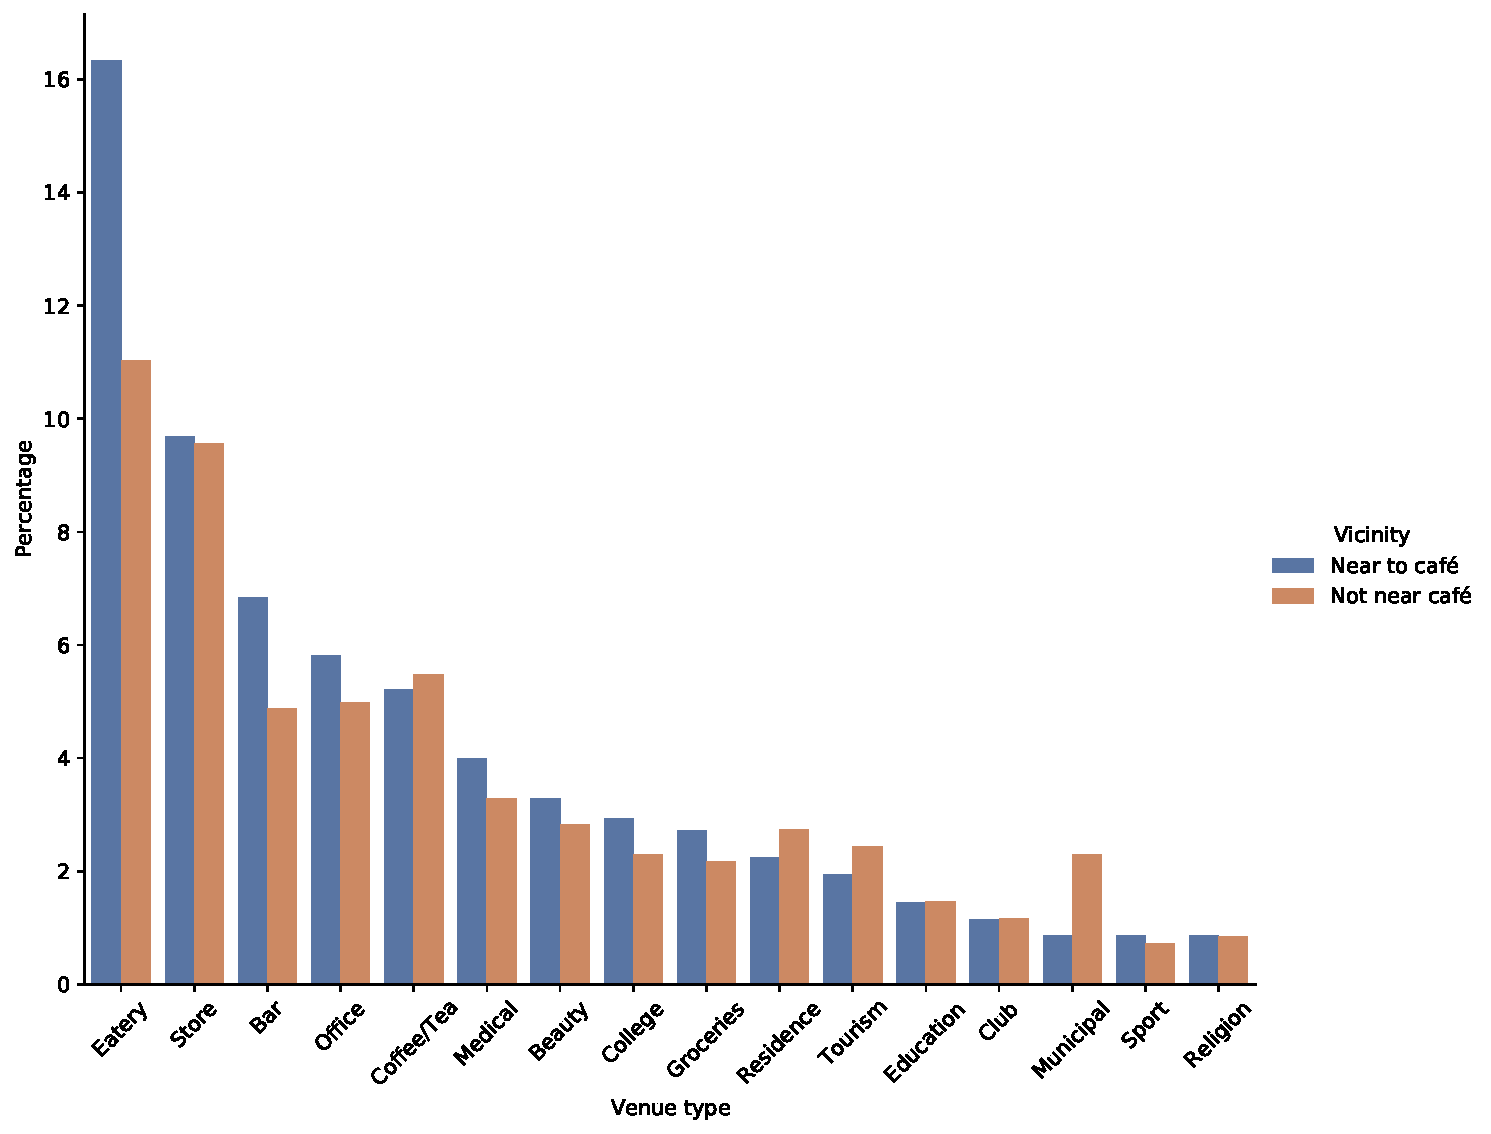
\includegraphics[width=0.85\textwidth]{avg_venues.pdf}
        \caption{\label{fig:AvgVenues}Comparison of the most common venue groups within vicinity of board game caf\'es and cities without. 
        We can see that areas near board game caf\'es contain a significant number more eating and drinking establishments, whereas city centres without include more municipal, residential and tourism-orientated buildings.}
    \end{figure}

    In order to get a general feel for areas where a board game caf\'e is located versus those where one is not, all of the encodings for the first category were grouped together, as were those from the second, and their means were again taken. 
    This left both the board game caf\'e areas and city areas with a single vector each of venue categories with each value now corresponding to the average percentage (as a decimal) for that given venue category over all for board game caf\'e and city areas, respectively.
    Because there were a lot of similar types, e.g. Italian Restaurant and French Restaurant, groupings of the most common venue categories (that is, taking over 55\% of all venue categories) were made and a comparison of these groupings was plotted (see Figure \ref{fig:AvgVenues}).\\

    The plot given in Figure \ref{fig:AvgVenues} suggests that whilst there are a lot of similarities between regions, e.g. in terms of stores, medical facilities and non-college education institutions, there are also some noticeable differences.
    These differences justify the decision to use venues as a determining factor for our decisions, as these are features that a classification model would be able to pick up on, and there is enough difference in land use between the districts of Turku.
    Of particular note are the differences in eateries, bars and municipal buildings, with areas near board game caf\'es having a much higher number of eating and drinking venues but much fewer official buildings.
    This is consistent with the idea that board game caf\'es are recreational venues, usually with food and alcohol licenses, so would be found in areas focus on nightlife and recreation.

    \subsection{Clustering of caf\'es and cities}

    We hypothesised that it may be possible to perform some clustering upon both the areas around board game caf\'es and the city centres without, to see if there were any commonalities between areas.
    However, upon applying a $\mathsf{K}$-means clustering model to both sets of data, it was found that for values of $\mathsf{K}$ between 2 and 20 (inclusive) the silhouette score for each never exceeded 0.08, and decreased with increasing $\mathsf{K}$. 
    Silhouette scores that close to zero (its maximum value is 1) suggest that the data points are lying on the boundaries of clusters, and the decreasing value means that they are nearing being within the wrong clusters altogether.
    This problem is likely due to the sparseness of the data: there 724 venue categories, and of those only a small number will have non-zero values for a given area (recall that we are only considering a circle of radius 400m), so it is likely very difficult to find suitable groupings.

    \section{Modelling}
    
    \begin{figure}[b]
        \centering
        \begin{tabular}{l | c | c | c}
            & Accuracy & Log loss & $\mathsf{F}_1$ score \\
            \hline
            Logistic Regression & 0.854 & 0.389 & 0.825 \\
            \hline
            Random Forest & 0.832 & 0.437 & 0.792 \\
            \hline
            Support Vector & 0.879 & 0.321 & 0.830 \\
            \hline
            Voting & 0.898 & 0.370 & 0.877
        \end{tabular}
        \captionof{table}{\label{tab:ModelComarison} Score comparison of the four models trained on our data.}
    \end{figure}

    The data was modelled using a collection of classification models: logistic regression, random forest, support vector machine and a voting classifier, which makes a decision based on the results of the other three.
    A cross-validated grid search was performed upon the logistic regression and support vector classifiers, with both having their normalisation coefficient $\mathsf{C}$ varied (over the range of values 0.01, 0.03, 0.1, 0.3, 1, 3), and logistic regression classifier having its solver varied.
    After training and testing both models on the training data (which had a train/test split of 80\%/20\%) the optimal value of $\mathsf{C}$ and solver for the logistic regression classifier were 0.3 and `liblinear', respectively, whilst the optimal value of $\mathsf{C}$ for the support vector classifier was 1.
    These were tested against a random forest classifier and a voting classifier that utilised information from all three to make an informed decision, with their accuracy, log loss and $\mathsf{F}_1$ score kept track of. 
    The results of these tests are given in Table \ref{tab:ModelComarison}.\\

    

    \begin{figure}[t]
        \centering
        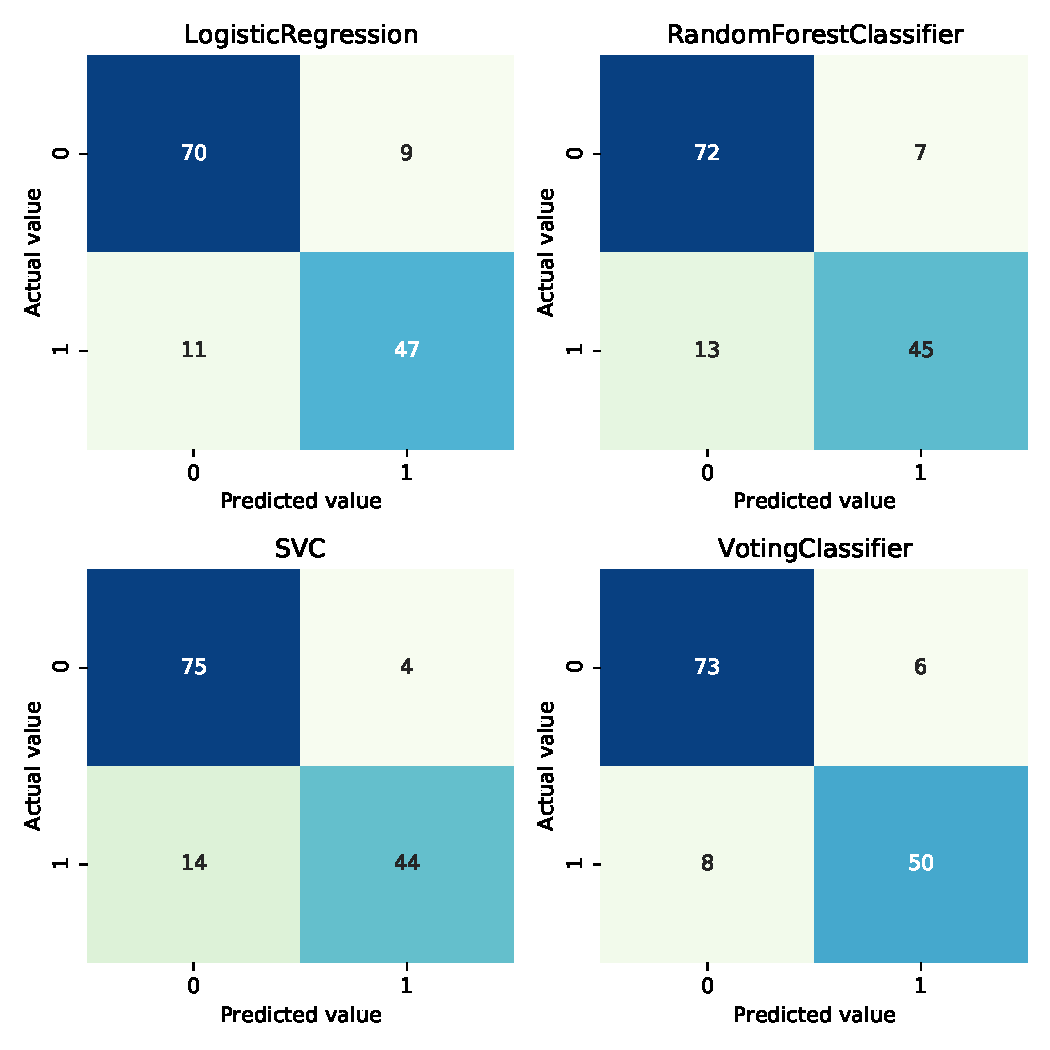
\includegraphics[width=0.6\textwidth]{model_comparison.pdf}
        \caption{\label{fig:ModelComparison}Comparison of the four classification models. 
        We can see that the voting classifier has the most true positives and fewest false negatives, whilst the support vector classifier has the most true negatives and the least false positives, with the logistic regression and random forest classifiers performing worse overall. 
        However, the false negative rate of the support vector classifier is far higher than the false positive rate of the voting classifier, so the latter is the better option.}
    \end{figure}

    In addition, a confusion matrix was plotted for the predictions of each model against the test data (see Figure \ref{fig:ModelComparison}).
    We can see from the confusion matrix and the table that the random forest classifier performed worst overall, with the second most false negatives and false positives. 
    The logistic regression classifier was the most `optimistic' model with the most false positives, whilst the support vector classifier was the most `pessimistic' with the most false negatives.
    Finally, the voting classifier, while not getting the most true negatives, was the most accurate overall and had the largest $\mathsf{F}_1$ score (and only slightly higher log loss than the support vector classifier).
    With these factors in mind, the voting classifier made sense as the model to apply to the Turku data, and its high accuracy and $\mathsf{F}_1$ score suggested it to be a good quality model.


    \section{Results}

    \begin{figure}[h]
        \centering
        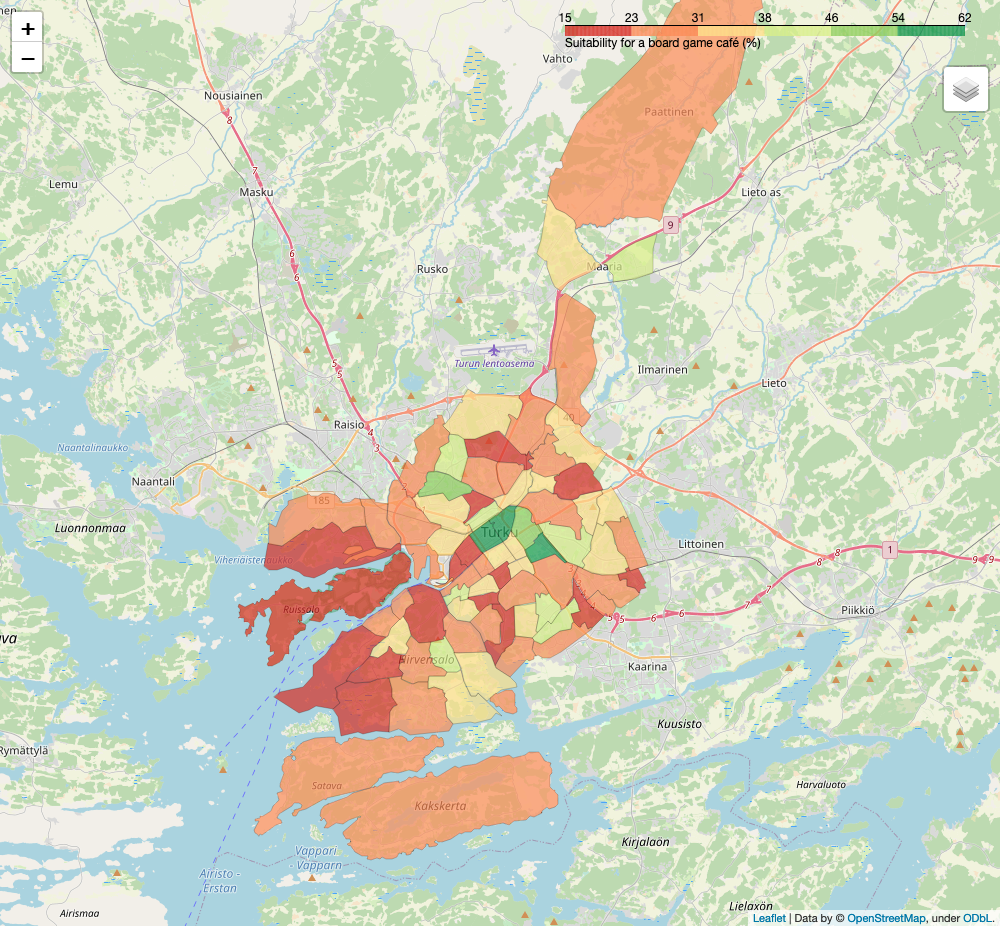
\includegraphics[width=0.8\textwidth]{Turku_map.png}
        \caption{\label{fig:Turkuprobs}The feasibility of each district of Turku. 
        Red and yellow regions would not make suitable candidates, whereas those in darker shades of green would be worth considering.}
    \end{figure}

    After applying the voting classifier model to the Turku venue data, each district obtained a probability corresponding to the model's confidence in the district belonging to the category of having a board game caf\'e, which we interpret here as its suitability for one. 
    These probabilities were, in collaboration with the region polygons for the districts of Turku, superimposed upon a map of the city as a choropleth (see Figure \ref{fig:Turkuprobs}).
    The probabilities were colour-coded, with red regions denoting areas of low suitability, and green being regions of higher.
    The locations considered suitable, with their corresponding probabilities, are given in Table \ref{tab:Suitability}. \\

    \begin{figure}[h]
        \centering
        \begin{tabular}{l | r }
            District & Probability of suitability\\
            \hline
            VI (Centre) & 61.93\% \\
            \hline
            Kupittaa & 58.87\% \\
            \hline
            VII (Centre) & 54.28\% \\
        \end{tabular}
        \captionof{table}{\label{tab:Suitability} Probabilities for districts of Turku predicted to be suitable for a board game caf\'e.}
    \end{figure}

    The districts VI and VII are perhaps not too surprising, given they are located within the very centre of the city, with a large number of restaurants and bars, as well large shopping establishments.
    Kupittaa, on the other hand, is less obvious, especially when to most residents in Turku it is known for containing a park, swimming pool and sports stadium.
    However, it also contains an area of high density tech offices, along with restaurants and a campus for the university of applied sciences.
    Given the venues contained within these districts, it would likely make sense that a board game caf\'e would be located in one of these. \\

    There are a few relatively surprising locations within the suburbs of Turku, namely Ruohonp\"a\"a and Peltola, that are also very close to the being suitable, with probabilities of 47.42\% and 42.73\% respectively. 
    However, both contain a high density of shopping facilities, with Ruohonp\"a\"a housing the L\"ansikeskus commercial region.

    \section{Conclusions}

    This study has investigated the suitability of districts within the city of Turku to support a board game caf\'e, based on classification models trained using venue data surrounding all board game caf\'es within Europe and the centres of cities that do not have such caf\'es. 
    By performing a comparison of the average venues within areas near to board game caf\'es and those that are not, we could see clear distinctions between the two, justifying the basis of this work.
    After running a comparison of several classification models, a voting classifier was chosen and was found to have both a high accuracy and $\mathsf{F}_1$ score, reducing the risk of false positives and negatives.
    By applying this model to our venue data for Turku three districts were considered suitable for supporting a board game caf\'e: VI, VII and Kupittaa.
    This information would provide prospective board game caf\'e owners the option to consider each district, see what spaces are available and find the one that best suits their needs and budget.\\

    This project was by no means exhaustive, and a logical next step would be to become more granular: now that three possible districts have been chosen, it would make sense to limit to those and consider which streets are best suited.
    This is most prevalent in Kupittaa, where almost every venue that would have impacted the decision lies on or adjacent to one road, namely Lemmink\"aisenkatu.
    In addition, providing more than one location in a given city as counterexample data would allow for richer features to be picked out by the model, as would examining additional features such as the average age or income of residents close to or in an area.
    However, the model as presented here provides an encouraging first step in this direction.



    \bibliographystyle{unsrt}

	\begin{thebibliography}{10}

		\bibitem{Meeple}
		Matthews,~A. (2019, December 27). The Ultimate Worldwide Guide to Board Game Cafes [Blog post]. Retrieved from \url{https://www.meeplemountain.com/articles/the-ultimate-guide-to-board-game-cafes/}

        \bibitem{MeepleMap}
        Worldwide Board Game Cafe List. Retrieved from \url{https://www.google.com/maps/d/u/0/viewer?mid=1UEkafkpKjbEJQzkcwgdtmnYPn4jXQKrw}

        \bibitem{CityMayors}
        City Mayors: The 500 largest European cities. Retrieved from \url{http://www.citymayors.com/features/euro_cities.html}

        \bibitem{WikiTurkey}
        List of largest cities and towns in Turkey. Retrieved from \url{https://en.wikipedia.org/wiki/List_of_largest_cities_and_towns_in_Turkey}

        \bibitem{WikiTurku}
        Districts of Turku. Retrieved from \url{https://en.wikipedia.org/wiki/Districts_of_Turku}

        \bibitem{WikiEU}
        List of sovereign states and dependent territories in Europe. Retrieved from \url{https://en.wikipedia.org/wiki/List_of_sovereign_states_and_dependent_territories_in_Europe#Sovereign_states}

	\end{thebibliography}

\end{document}